\documentclass{article}
\usepackage[utf8]{inputenc}
\usepackage[margin=1.5cm, top=2cm, bottom=2cm]{geometry}
\usepackage{amsmath}
\usepackage{amsfonts}
\usepackage{amssymb}
\usepackage{graphicx}
\usepackage{setspace}
\setstretch{0.9}

\title{CS229 Notes - June 26, 2025}
\author{Yuren Hao}
\date{\today}

\begin{document}

\maketitle

\section{Maximum Likelihood Estimation (MLE)}

Given i.i.d. observations $x_1, x_2, \ldots, x_n$ from $f(x; \theta)$.

\textbf{Likelihood:} $L(\theta) = \prod_{i=1}^{n} f(x_i; \theta)$

\textbf{Log-likelihood:} $\ell(\theta) = \sum_{i=1}^{n} \log f(x_i; \theta)$

\textbf{MLE:} $\hat{\theta}_{MLE} = \arg\max_{\theta} \ell(\theta)$

Solve: $\frac{\partial \ell(\theta)}{\partial \theta} = 0$

\section{Linear Regression - Normal Equation}

Given training data $\{(x_i, y_i)\}_{i=1}^n$ with $x_i \in \mathbb{R}^d$, $y_i \in \mathbb{R}$.

\textbf{RSS:} $RSS(\theta) = \sum_{i=1}^{n} (y_i - \theta^T x_i)^2 = \|y - X\theta\|_2^2$

\textbf{Derivative:} $\frac{\partial RSS(\theta)}{\partial \theta} = -2X^T(y - X\theta)$

\textbf{Normal Equation:} $X^TX\theta = X^Ty$

\textbf{Closed-form solution:} $\hat{\theta} = (X^TX)^{-1}X^Ty$

\section{Gradient Descent for Linear Regression}

\textbf{Cost function:} $J(\theta) = \frac{1}{2m}\sum_{i=1}^{m} (h_\theta(x^{(i)}) - y^{(i)})^2$

\textbf{Gradient:} $\frac{\partial J}{\partial \theta_j} = \frac{1}{m}\sum_{i=1}^{m} (h_\theta(x^{(i)}) - y^{(i)})x_j^{(i)}$

\textbf{Algorithm:}
\begin{enumerate}
    \item Initialize $\theta$ randomly
    \item While not converged:
    \begin{itemize}
        \item $\theta_j := \theta_j - \alpha \frac{\partial J}{\partial \theta_j}$ for all $j$
        \item Check convergence: $|J(\theta^{(t+1)}) - J(\theta^{(t)})| < \epsilon$
    \end{itemize}
\end{enumerate}

\textbf{Vectorized update:} $\theta := \theta - \alpha \frac{1}{m} X^T(X\theta - y)$

\subsection{Example: 3 Data Points}
\textbf{Data:} $(1,1)$, $(2,2)$, $(3,4)$. Model: $h_\theta(x) = \theta_0 + \theta_1 x$

\textbf{Initial:} $\theta_0 = 0$, $\theta_1 = 0$, $\alpha = 0.1$

\textbf{Iteration 1:}
\begin{itemize}
    \item $J(\theta) = \frac{1}{6}[(0-1)^2 + (0-2)^2 + (0-4)^2] = 3.5$
    \item $\frac{\partial J}{\partial \theta_0} = \frac{1}{3}[(-1) + (-2) + (-4)] = -2.33$
    \item $\frac{\partial J}{\partial \theta_1} = \frac{1}{3}[(-1)(1) + (-2)(2) + (-4)(3)] = -5.67$
    \item $\theta_0 := 0 - 0.1(-2.33) = 0.233$
    \item $\theta_1 := 0 - 0.1(-5.67) = 0.567$
\end{itemize}

\textbf{Iteration 2:} $J(\theta) = 1.26$ (continues until convergence...)

\section{ML Framework \& Loss Functions}

\subsection{General ML Pipeline}
\textbf{Model} $\rightarrow$ \textbf{Algorithm} $\rightarrow$ \textbf{Estimated Parameters}

\textbf{Predictions} $\rightarrow$ \textbf{Decisions} $\rightarrow$ \textbf{Outcomes}

\textbf{Example:} Linear model $\rightarrow$ Gradient descent $\rightarrow$ $\hat{\theta}$

House price prediction $\rightarrow$ Buy/sell decision $\rightarrow$ Profit/loss

\subsection{Loss Functions}
\textbf{Regression:}
\begin{itemize}
    \item \textbf{MSE:} $L(y, \hat{y}) = (y - \hat{y})^2$
    \item \textbf{MAE:} $L(y, \hat{y}) = |y - \hat{y}|$
    \item \textbf{Huber:} $L(y, \hat{y}) = \begin{cases} \frac{1}{2}(y-\hat{y})^2 & \text{if } |y-\hat{y}| \leq \delta \\ \delta|y-\hat{y}| - \frac{1}{2}\delta^2 & \text{otherwise} \end{cases}$
\end{itemize}

\textbf{Classification:}
\begin{itemize}
    \item \textbf{0-1 Loss:} $L(y, \hat{y}) = \mathbf{1}[y \neq \hat{y}]$
    \item \textbf{Logistic:} $L(y, \hat{y}) = -y\log(\hat{y}) - (1-y)\log(1-\hat{y})$
    \item \textbf{Hinge:} $L(y, \hat{y}) = \max(0, 1 - y\hat{y})$ (SVM)
\end{itemize}

\section{Training Loss vs Model Complexity}

\subsection{Bias-Variance Tradeoff}
\textbf{Low Complexity:} High bias, low variance $\rightarrow$ \textbf{Underfitting}

\textbf{High Complexity:} Low bias, high variance $\rightarrow$ \textbf{Overfitting}

\subsection{Typical Curves}
\begin{itemize}
    \item \textbf{Training Error:} Decreases as complexity increases
    \item \textbf{Validation Error:} U-shaped curve
    \item \textbf{Optimal Complexity:} Minimum validation error
\end{itemize}

\begin{figure}[h]
\centering
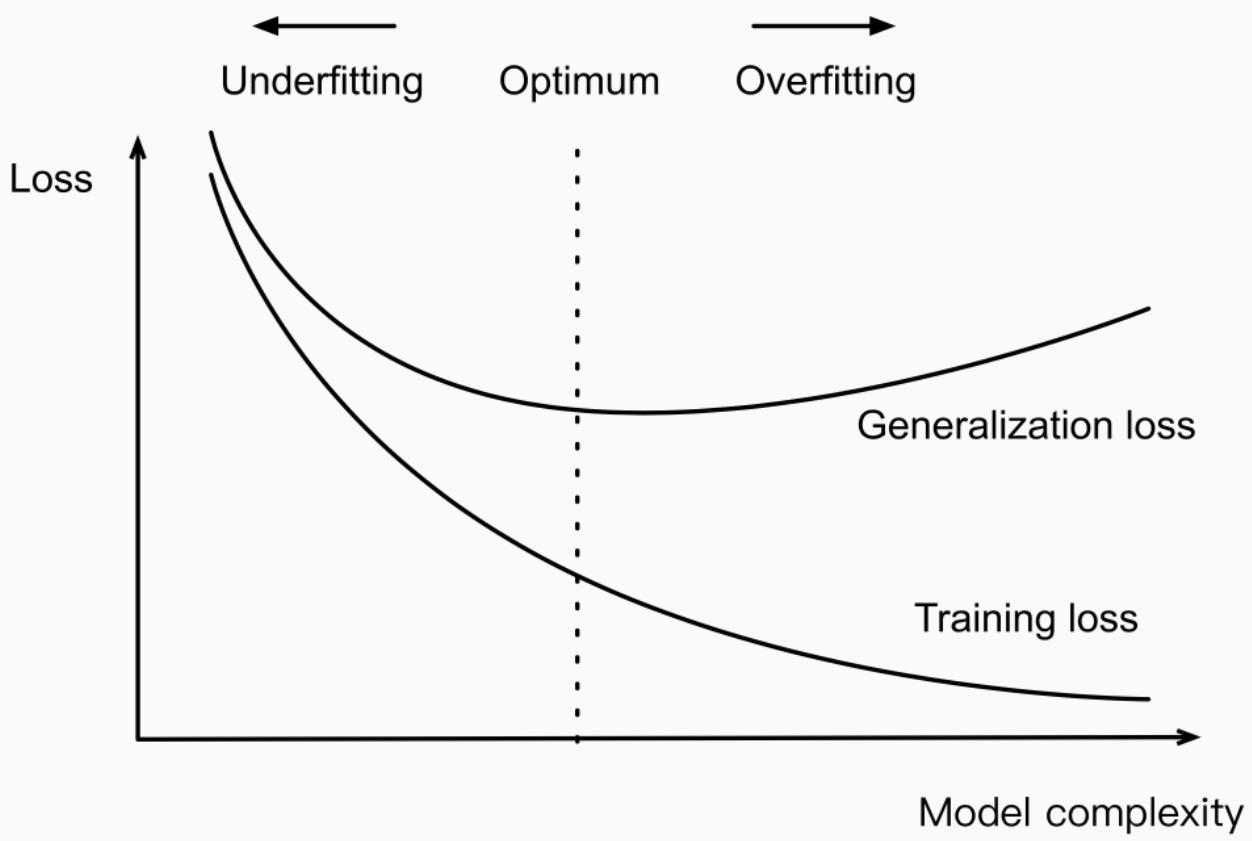
\includegraphics[width=0.8\textwidth]{model-complexity-diagram.png}
\caption{Model Complexity vs Training/Validation Error}
\end{figure}

\textbf{Total Error} = Bias$^2$ + Variance + Irreducible Error

\textbf{Regularization:} Controls complexity via penalty terms
\begin{itemize}
    \item \textbf{L1 (Lasso):} $\lambda \sum_j |\theta_j|$ (sparse solutions)
    \item \textbf{L2 (Ridge):} $\lambda \sum_j \theta_j^2$ (smooth solutions)
\end{itemize}

\section{Generalization Error}

\subsection{Definition}
\textbf{Generalization Error:} Expected error on unseen data from same distribution

\textbf{Continuous Case:} For regression with squared loss
\[
\text{Gen Error} = \mathbb{E}_{(x,y) \sim D}[(h(x) - y)^2] = \int_{x,y} (h(x) - y)^2 p(x,y) \, dx \, dy
\]

If $p(x,y) = p(y|x)p(x)$, then:
\[
= \int_x \left[ \int_y (h(x) - y)^2 p(y|x) \, dy \right] p(x) \, dx
\]

\textbf{Discrete Case:} For classification with 0-1 loss
\[
\text{Gen Error} = \mathbb{E}_{(x,y) \sim D}[\mathbf{1}[h(x) \neq y]] = \sum_{x,y} \mathbf{1}[h(x) \neq y] \cdot p(x,y)
\]

Expanding the sum:
\[
= \sum_x \sum_{y: y \neq h(x)} p(x,y) = \sum_x p(x) \sum_{y: y \neq h(x)} p(y|x)
\]

Where $D$ is the data distribution, $h$ is the hypothesis

\textbf{Empirical Risk:} Approximation using training data

\textbf{Continuous Case:}
\[
\hat{R}(h) = \frac{1}{m}\sum_{i=1}^{m} (h(x_i) - y_i)^2
\]

\textbf{Discrete Case:}
\[
\hat{R}(h) = \frac{1}{m}\sum_{i=1}^{m} \mathbf{1}[h(x_i) \neq y_i]
\]

\textbf{General Form:}
\[
\hat{R}(h) = \frac{1}{m}\sum_{i=1}^{m} L(h(x_i), y_i) \approx \mathbb{E}_{(x,y) \sim D}[L(h(x), y)]
\]

\textbf{Generalization Gap:} $R(h) - \hat{R}(h)$ where $R(h)$ is true risk

\subsection{Sources of Error}
The expected prediction error can be decomposed into three fundamental components:

\textbf{Expected Prediction Error:}
\[
\mathbb{E}[\text{Error}(x)] = \text{Noise} + \text{Bias}^2 + \text{Variance}
\]

\textbf{Detailed Breakdown:}
\begin{itemize}
    \item \textbf{Noise:} $\sigma^2 = \mathbb{E}[(y - f(x))^2]$ - Irreducible error from data
    \item \textbf{Bias:} $\text{Bias}[\hat{f}(x)] = \mathbb{E}[\hat{f}(x)] - f(x)$ - Model's systematic error
    \item \textbf{Variance:} $\text{Var}[\hat{f}(x)] = \mathbb{E}[(\hat{f}(x) - \mathbb{E}[\hat{f}(x)])^2]$ - Model's sensitivity to training data
\end{itemize}

\textbf{MSE Decomposition:}
\[
\text{MSE}(x) = \mathbb{E}[(\hat{f}(x) - y)^2] = \text{Bias}^2[\hat{f}(x)] + \text{Var}[\hat{f}(x)] + \sigma^2
\]

Expanding the MSE:
\[
= (\mathbb{E}[\hat{f}(x)] - f(x))^2 + \mathbb{E}[(\hat{f}(x) - \mathbb{E}[\hat{f}(x)])^2] + \mathbb{E}[(y - f(x))^2]
\]

\textbf{Experimental Setup for Bias-Variance Analysis:}

We create $N$ different training sets by sampling from the data distribution. Each training set produces estimated model parameters, giving us $N$ different models $\hat{f}_1, \hat{f}_2, \ldots, \hat{f}_N$.

Use the average predictions of all the $N$ estimated models, denoted by $\bar{f}_w(x)$:
\[
\bar{f}_w(x) = \frac{1}{N}\sum_{i=1}^{N} \hat{f}_i(x)
\]

The average fit is akin to the expected prediction $\mathbb{E}[\hat{f}(x)]$ over all possible training sets.

\textbf{Bias Definition:}
\[
\text{Bias}(x) = f_{\text{true}}(x) - \bar{f}_w(x)
\]

\textbf{Key Question:} Is our approach flexible enough to capture $f_{\text{true}}(x)$?

Bias is high when the hypothesis class is unable to capture $f_{\text{true}}(x)$. This happens when the model class is too simple or restrictive to represent the true underlying function.

\textbf{Model Complexity vs Bias-Variance:}

\textbf{Low Complexity Model:}
\begin{itemize}
    \item \textbf{High Bias} - Cannot capture complex patterns in $f_{\text{true}}(x)$
    \item \textbf{Low Variance} - Predictions consistent across different training sets
    \item Example: Linear model for non-linear data
\end{itemize}

\textbf{High Complexity Model:}
\begin{itemize}
    \item \textbf{Low Bias} - Can approximate $f_{\text{true}}(x)$ well
    \item \textbf{High Variance} - Predictions vary significantly with training data
    \item Example: High-degree polynomial or deep neural network
\end{itemize}

\textbf{Key Insight:} There's a fundamental tradeoff - reducing bias often increases variance, and vice versa.

\begin{figure}[h]
\centering
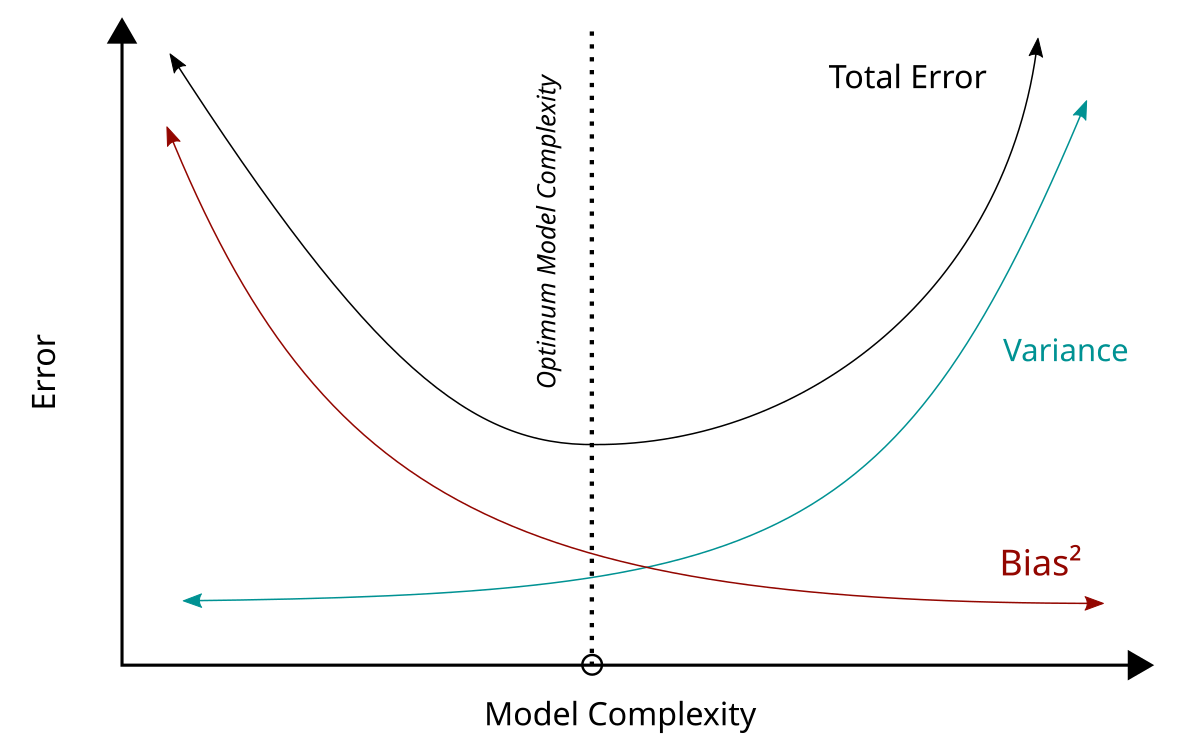
\includegraphics[width=0.85\textwidth]{bias-variance-diagram.png}
\caption{Bias and Variance Contributing to Total Error (Source: Wikimedia Commons)}
\end{figure}

\subsection{Approximating Generalization Error}
Since true distribution $D$ is unknown, we approximate generalization error using:
\textbf{Validation Set:} Hold-out data to estimate $R(h) \approx \hat{R}_{val}(h)$
\textbf{Cross-Validation:} Average over multiple train/validation splits to reduce variance.
The key insight: empirical risk on unseen validation data provides unbiased estimate of generalization error.

\subsection{Test Error Definition}
\textbf{Test Error:} Performance on final held-out test set, used only once for final evaluation.

\textbf{Continuous Case (Regression):}
\[
\text{Test Error} = \frac{1}{n_{test}}\sum_{i=1}^{n_{test}} (h(x_i^{test}) - y_i^{test})^2
\]

Expanding the sum:
\[
= \frac{1}{n_{test}}\left[ (h(x_1^{test}) - y_1^{test})^2 + (h(x_2^{test}) - y_2^{test})^2 + \ldots + (h(x_{n_{test}}^{test}) - y_{n_{test}}^{test})^2 \right]
\]

\textbf{Discrete Case (Classification):}
\[
\text{Test Error} = \frac{1}{n_{test}}\sum_{i=1}^{n_{test}} \mathbf{1}[h(x_i^{test}) \neq y_i^{test}]
\]

Expanding the indicator sum:
\[
= \frac{1}{n_{test}}\left[ \mathbf{1}[h(x_1^{test}) \neq y_1^{test}] + \mathbf{1}[h(x_2^{test}) \neq y_2^{test}] + \ldots + \mathbf{1}[h(x_{n_{test}}^{test}) \neq y_{n_{test}}^{test}] \right]
\]

\textbf{Key Point:} Test set should only be used once to avoid overfitting to test data.

\subsection{Key Factors}
\begin{itemize}
    \item \textbf{Model Complexity:} More parameters $\rightarrow$ higher capacity to overfit
    \item \textbf{Training Set Size:} More data $\rightarrow$ better generalization
    \item \textbf{Regularization:} Penalty terms reduce overfitting
    \item \textbf{Early Stopping:} Stop training before overfitting occurs
\end{itemize}

\end{document} 